% 简洁风格：浅色背景 + 细边框 + 行号 + 自动换行
\definecolor{codebg}{RGB}{248,249,250}
\definecolor{codeframe}{RGB}{220,223,228}
\definecolor{codekw}{RGB}{25,85,145}
\definecolor{codecm}{RGB}{90,125,90}
\definecolor{codestr}{RGB}{136,44,136}

\lstdefinestyle{cleancpp}{
	language=C++,
	basicstyle=\ttfamily\small,
	keywordstyle=\bfseries\color{codekw},
    commentstyle=\color{codecm},
	stringstyle=\color{codestr},
	backgroundcolor=\color{codebg},
	frame=single,
	rulecolor=\color{codeframe},
	framesep=6pt,
	numbers=left,
	numberstyle=\scriptsize\color{gray},
	numbersep=8pt,
	breaklines=true,
	breakatwhitespace=false,
	showstringspaces=false,
	keepspaces=true,
	tabsize=4,
	columns=fullflexible
}

\chapter{Exercise 4.1}

\section{Problem}

Given the following grammar:

\[
S \to (L) \;|\; a
\]
\[
L \to L , S \;|\; S
\]

Tasks:
\begin{enumerate}
	\item Eliminate left recursion in the grammar.
	\item Draw the transition diagrams for the grammar
	\item Write recursive-descent (predictive) procedures for the grammar.
	\item Indicate the procedure call sequence for the input sentence ``(a,(a,a))".
\end{enumerate}

\section{Solution}

\subsection{Eliminate left recursion}

The nonterminal $L$ is left-recursive. We rewrite $L$ as a right-recursive list (as shown):

\[
S \to (L) \;|\; a
\]
\[
L \to S L' \\
\]
\[
L' \to ,\;S\;L' \;|\; \epsilon
\]

The start production for $S$ remains $S\to (L)\;|\;a$.

\subsection{Draw the transition diagrams for the grammar}

The transition diagrams for the grammar are as follows:

\begin{figure}[htbp]
	\centering
	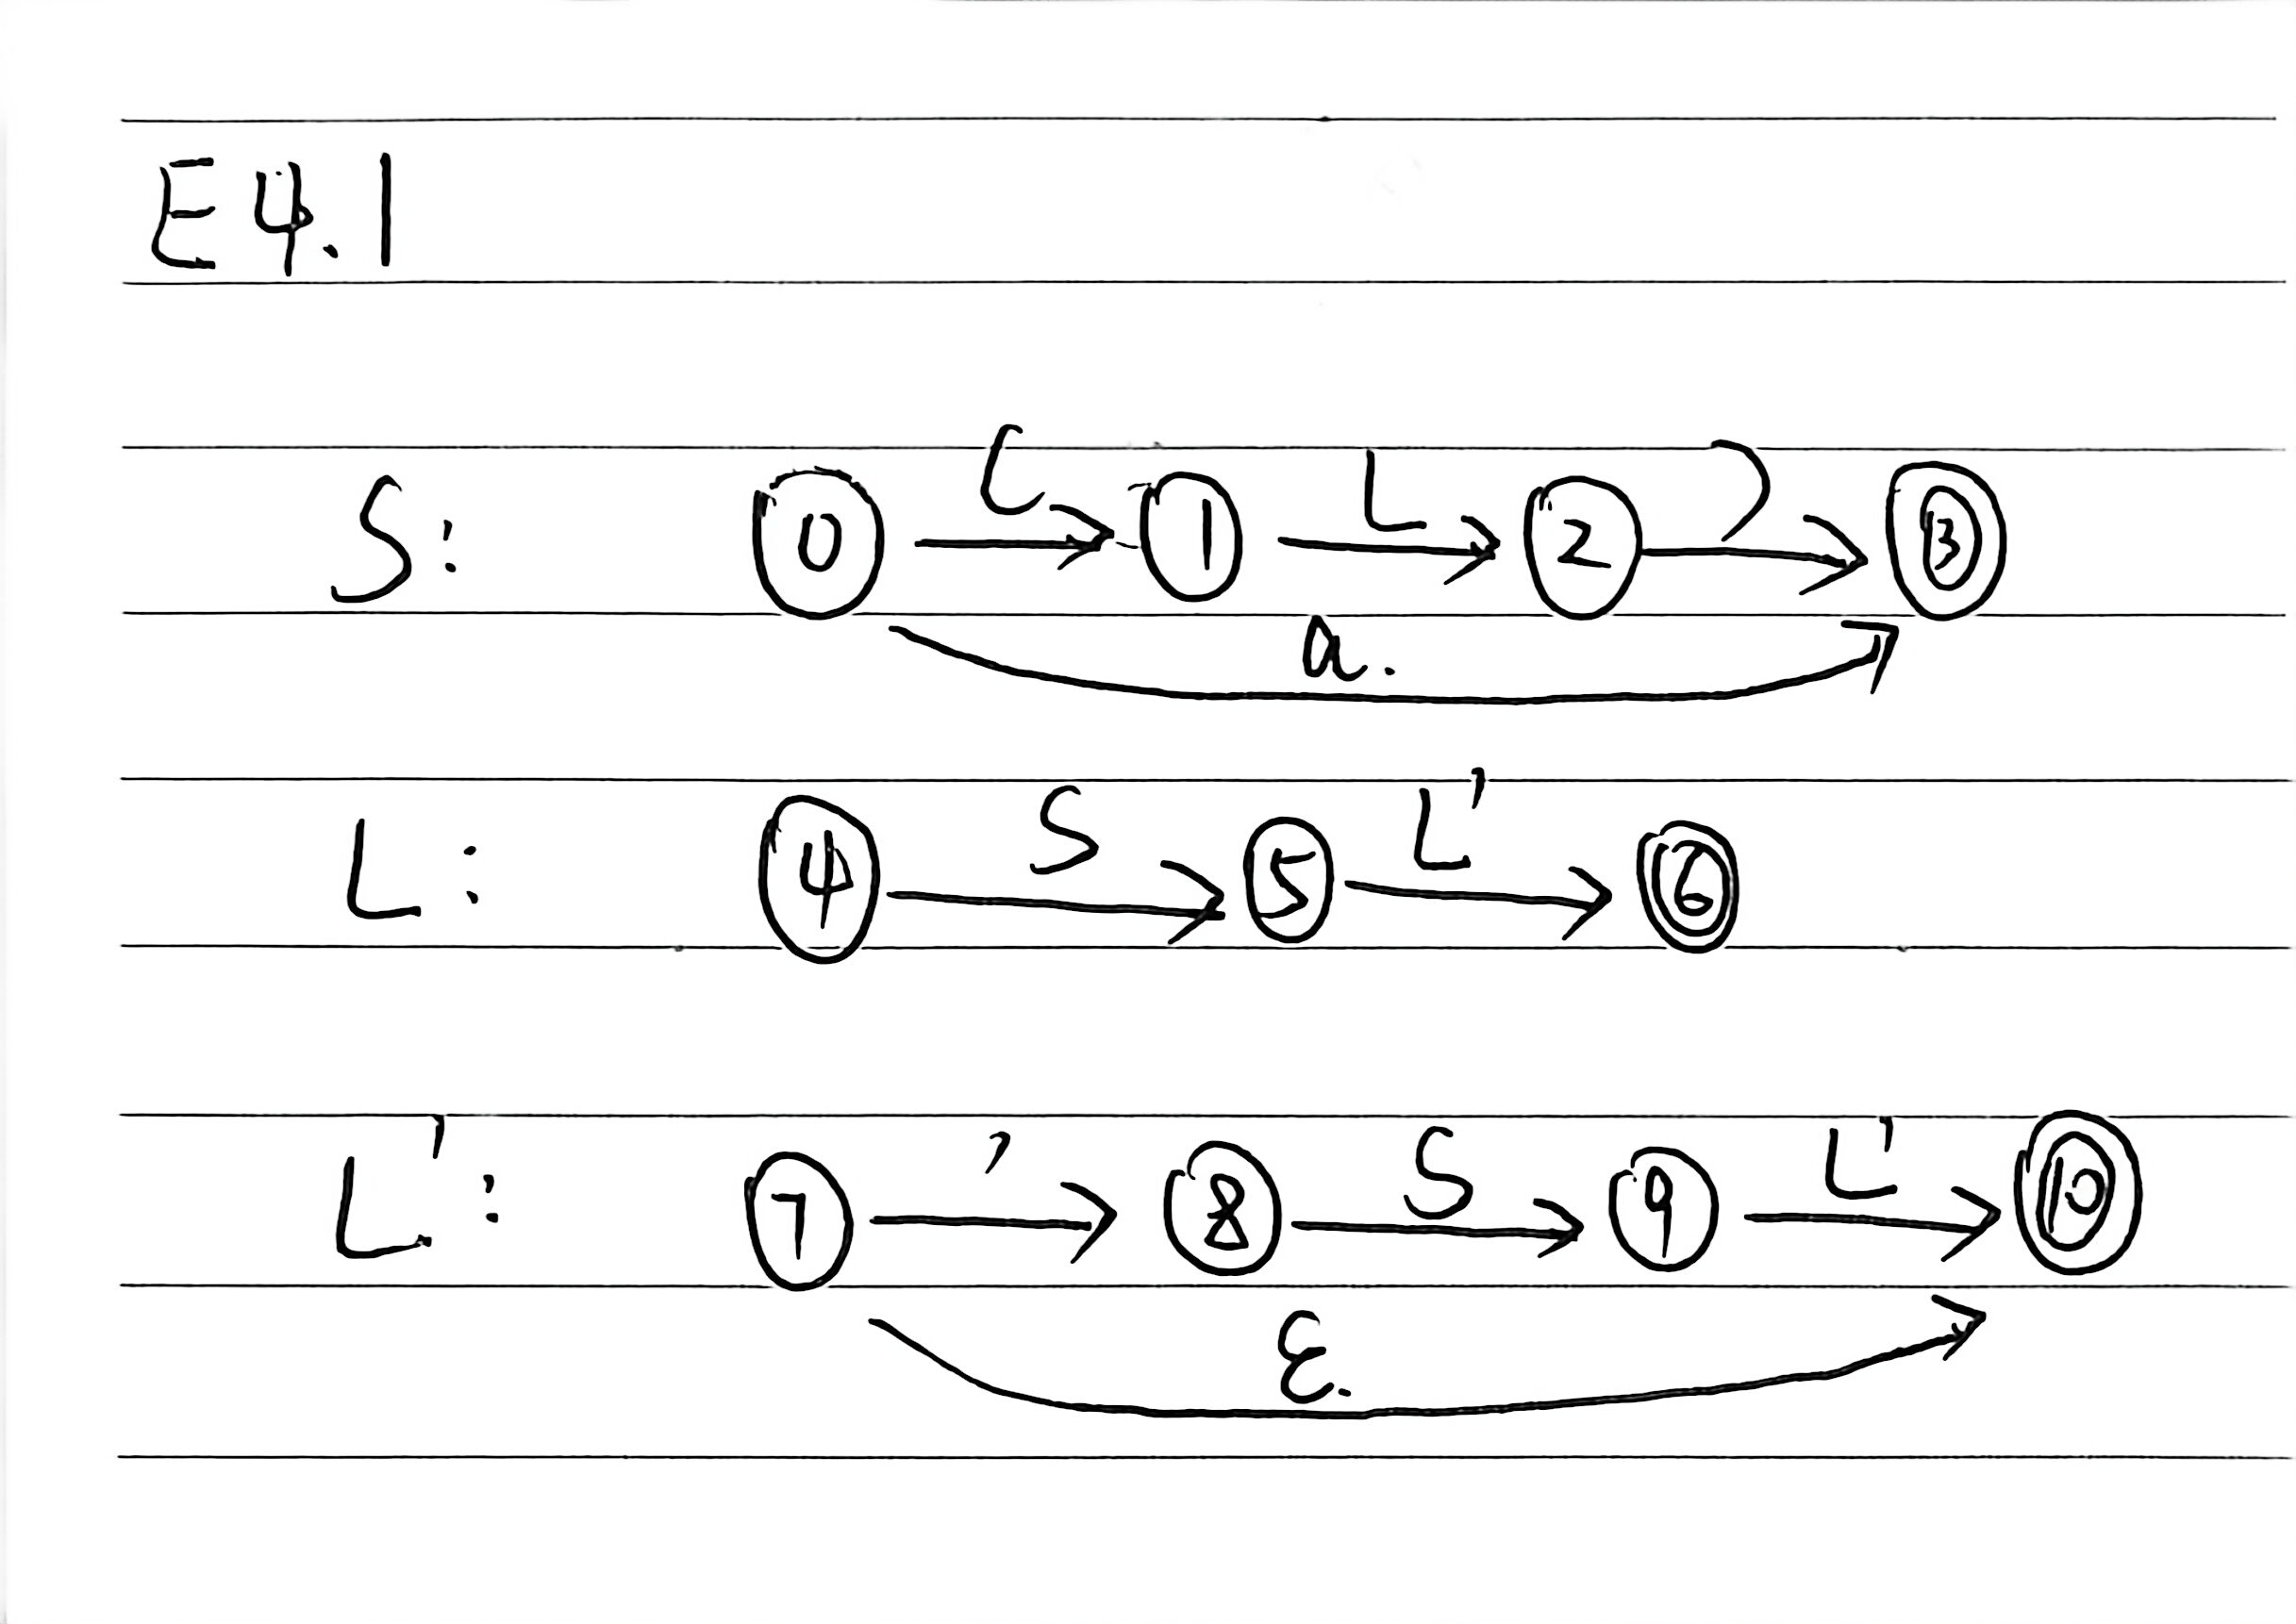
\includegraphics[width=\textwidth]{image/e4_1.JPG}
\end{figure}

\subsection{Predictive recursive-descent procedures (pseudocode)}

There are three procedures corresponding to the nonterminals $S$, $L$, and $L'$. Each procedure uses the lookahead token to decide which production to apply.

AS for S:
\begin{lstlisting}[style=cleancpp]
void S( ) {
    if ( lookahead == '(' ) {
        match( '(' );
        L( );
        match( ' )' );
    } 
    else if ( lookahead == a ) {
        match( a );
    } 
    else{
        error( );
    }
}
\end{lstlisting}

AS for L':
\begin{lstlisting}[style=cleancpp]
void L1( ) {
    if ( lookahead == ',' ) {
        match( ',' );
        S( );
        L1( );
    } 
    else if ( lookahead in FOLLOW(L') ) {
    }
    else{
        error( );
    }
}
\end{lstlisting}

AS for L:
\begin{lstlisting}[style=cleancpp]
void L1( ) {
    S();
    L1();
}
\end{lstlisting}

% \subsection{Procedure call sequence for the input ``(a,(a,a))"}
% 设初始输入为 \texttt{( a , ( a , a ) )}，初始时 \texttt{lookahead='('}。

% \begin{enumerate}
% 	\item 调用 \texttt{S()}：匹配 \texttt{'('}，此时 \texttt{lookahead = 'a'}。
% 	\item 递归调用 \texttt{L()}（处理列表）。
% 	\item 递归调用 \texttt{S()}：匹配 \texttt{a}，返回后 \texttt{lookahead = ','}。
% 	\item 回到步骤 2 中的 \texttt{L()}，见到 \texttt{','}，匹配 \texttt{','}，此时 \texttt{lookahead = '('}。
% 	\item 递归调用 \texttt{S()}：匹配 \texttt{'('}，此时 \texttt{lookahead = 'a'}。
% 	\item 递归调用 \texttt{L()}（处理内层列表）。
% 	\item 递归调用 \texttt{S()}：匹配 \texttt{a}，返回后 \texttt{lookahead = ','}。
% 	\item 回到步骤 6 中的 \texttt{L()}，递归调用 \texttt{L()}，匹配 \texttt{','}，此时 \texttt{lookahead = 'a'}，继续处理后续的 \texttt{S()}。
% 	\item 递归调用 \texttt{S()}：匹配 \texttt{a}，返回后 \texttt{lookahead = ')'}。
% 	\item 回到步骤 6 中的 \texttt{L()}，递归调用 \texttt{L()}，此时 \texttt{')'} 在 \texttt{FOLLOW(L)} 中，故对 \texttt{L'} 不做进一步匹配（即归约为 $\epsilon$）。
% 	\item 回到步骤 5 的 \texttt{S()}，匹配闭合的 \texttt{')'}，此时内层的 \texttt{S} 完成，\texttt{lookahead = ','}（返回到外层列表）。
% 	\item 回到步骤 2 的外层 \texttt{L()}，继续按规则处理，最终回到步骤 1 的 \texttt{S()}，匹配外层的闭合 \texttt{')'}，整个输入匹配成功，\texttt{S()} 返回，解析结束。
% \end{enumerate}

\subsection{Procedure call sequence for the input ``(a,(a,a))"}
Initial input: \texttt{( a , ( a , a ) )}, initial \texttt{lookahead='('}.

\begin{enumerate}
	\item Call \texttt{S()}: match \texttt{'('}; now \texttt{lookahead='a'}.
	\item Call \texttt{L()} to parse the list.
	\item Call \texttt{S()}: match \texttt{a}; now \texttt{lookahead=','}.
	\item Back in outer \texttt{L()}, see \texttt{','}: match it; now \texttt{lookahead='('}.
	\item Call \texttt{S()}: match \texttt{'('}; now \texttt{lookahead='a'} (enter inner list).
	\item Call inner \texttt{L()}.
	\item Call \texttt{S()}: match \texttt{a}; now \texttt{lookahead=','}.
	\item In inner \texttt{L()}, see \texttt{','}: match it and call \texttt{S()} for the next element.
	\item Call \texttt{S()}: match \texttt{a}; now \texttt{lookahead=')'}.
	\item In inner \texttt{L()}, \texttt{')'} is in FOLLOW(L), so \texttt{L'} -> \(\epsilon\) (no further matches).
	\item Return to inner \texttt{S()}: match closing \texttt{')'}; inner \texttt{S} completes; now \texttt{lookahead=','} (back to outer list).
	\item Continue outer \texttt{L()}, then return to outer \texttt{S()} and match closing \texttt{')'}; input accepted.
\end{enumerate}

\chapter{Exercise 4.2}

\section{Problem}

Consider the context-free grammar

\[
S \to a S b S \;|\; b S a S \;|\; \epsilon
\]

Can you construct a predictive (LL(1)) parser for this grammar? Explain why or why not.

\section{Solution}

No, we cannot construct a predictive (LL(1)) parser for this grammar. The grammar is ambiguous because the same string can be derived in multiple ways. For example, the string "ab" can be derived as follows:
\[S \to a S b S \to a \epsilon b \epsilon = ab
\]
or
\[S \to b S a S \to b \epsilon a \epsilon = ba
\]

\chapter{Exercise 4.3}

\section{Problem}

Compute the FIRST and FOLLOW for the start symbol of the following grammar:

\[
S \to S\;S\;+ \;|\; S\;S\;* \;|\; a
\]

\section{Solution}

\subsection{Eliminate Left Recursion}

The given grammar contains left recursion. To eliminate it, we rewrite the grammar as follows:

\[
S \to aS' 
\]
\[
S' \to S+S' \;|\; S*S' \;|\; \epsilon
\]

\subsection{Left Factoring}

To make the grammar suitable for predictive parsing, we perform left factoring:

\[
S \to aS' 
\]
\[
S' \to S T \;|\; \epsilon
\]
\[
T \to +S' \;|\; *S'
\]

\subsection{FIRST and FOLLOW Sets}

The FIRST and FOLLOW sets for the start symbol $S$ are computed as follows:

\[
\text{FIRST}(S) = \{a\}
\]
\[
\text{FOLLOW}(S) = \{+, *, \$\}
\]
